\section{建立连接过程}
\subsection{简述建立连接过程}
MPTCP依然按照正常的TCP进行三次握手,只是在握手过程中增加了MPTCP特有的信息,三次握手过程如下图~\ref{label:建立连接过程}:
\begin{figure}[H]
  \centering
  % Requires \usepackage{graphicx}
  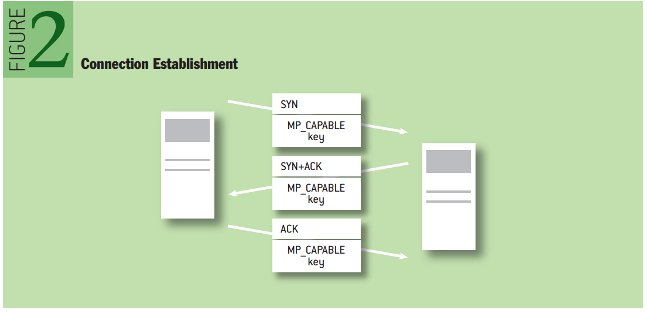
\includegraphics[width=10cm]{dias/Connection_Establishment.jpg}\\
  \caption{建立连接过程}
  \label{label:建立连接过程}
\end{figure}
左边客户端发送的第一个SYN包携带有客户端自身的KEY,右边发送SYN/ACK的时候携带了自身的KEY,而最后左边的客户端发送最后一个ACK的时候携带着双方的KEY。MPTCP中关于MP\_CAPABLE的定义如图~\ref{label:MPCAPABLE的定义}:
\begin{figure}[H]
  \centering
  % Requires \usepackage{graphicx}
  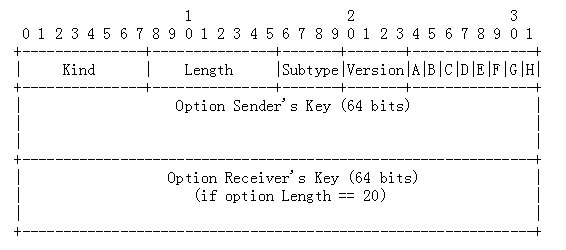
\includegraphics[width=10cm]{dias/Definition_of_MP_CAPABLE.jpg}\\
  \caption{MP\_CAPABLE的定义}
  \label{label:MPCAPABLE的定义}
\end{figure}

\begin{figure}[H]
  \centering
  % Requires \usepackage{graphicx}
  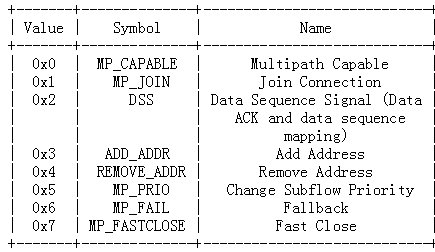
\includegraphics[width=10cm]{dias/Definition_of_Subtype.jpg}\\
  \caption{Subtype的定义}
  \label{fig:Subtype的定义}
\end{figure}

\subsection{建立连接过程的内核实现}
MPTCP在客户端上发送SYN包的调用情况如下:
\begin{figure}[H]
  \centering
  % Requires \usepackage{graphicx}
  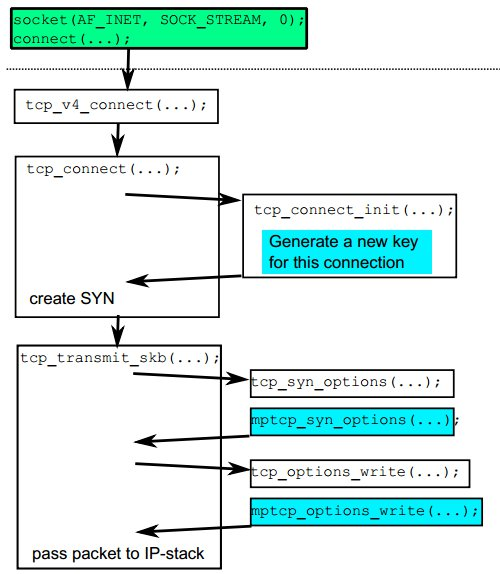
\includegraphics[width=10cm]{dias/Invoke_SYN_in_Cilent.jpg}\\
  \caption{客户端上发送SYN包的调用情况}
\end{figure}
关键函数为mptcp\_syn\_options对MPTCP选项的填充,源码如下:
\small\begin{verbatim}
"net/mptcp/mptcp_output.c" line 843 of 1667
843 void mptcp_syn_options(struct sock *sk, struct tcp_out_options *opts,unsigned *remaining)
845 {
846     struct tcp_sock *tp = tcp_sk(sk);
847
848     opts->options |= OPTION_MPTCP;
849     if (is_master_tp(tp)) {
850         opts->mptcp_options |= OPTION_MP_CAPABLE | OPTION_TYPE_SYN;
851         *remaining -= MPTCP_SUB_LEN_CAPABLE_SYN_ALIGN;
852         opts->mp_capable.sender_key = tp->mptcp_loc_key;
853         opts->dss_csum = !!sysctl_mptcp_checksum;
854     } else {
855         struct mptcp_cb *mpcb = tp->mpcb;
856
857         opts->mptcp_options |= OPTION_MP_JOIN | OPTION_TYPE_SYN;
858         *remaining -= MPTCP_SUB_LEN_JOIN_SYN_ALIGN;
859         opts->mp_join_syns.token = mpcb->mptcp_rem_token;
860         opts->mp_join_syns.low_prio  = tp->mptcp->low_prio;
861         opts->addr_id = tp->mptcp->loc_id;
862         opts->mp_join_syns.sender_nonce = tp->mptcp->mptcp_loc_nonce;
863     }
864 }
\end{verbatim}\normalsize
由于三次握手的肯定是master sock,在850行到853行对MPTCP选项进行了赋值。相应的服务端发送SYN/ACK包时使用mptcp\_synack\_options 函数对选项进行了赋值。而最后一个ACK包则是调用函数mptcp\_established\_options操作。
\subsection{结论}
\begin{itemize}
  \item MPTCP利用TCP的三次握手进行了KEY信息的交换。
\end{itemize}